\documentclass[a4paper,10pt]{article}
\usepackage[utf8]{inputenc}
\usepackage{graphicx}
\usepackage{amsmath}
\usepackage{amssymb}
\usepackage{amsthm}
\usepackage{booktabs}
\usepackage{caption}
\usepackage{geometry}
%\usepackage{hyperref}
\usepackage{makeidx}
\usepackage{microtype}
\usepackage{subfig}
\usepackage{tabularx}
\usepackage{url}
\usepackage{varioref}
\usepackage[italian]{babel}
\usepackage{xcolor}
\usepackage{multicol}
\usepackage{mathtools}
\usepackage{booktabs}
\usepackage{gensymb}


\title{Laboratorio I: Pendolo quadrifilare\\ Misura del periodo.\\
\begin{large}
Dipartimento di Fisica E.Fermi - Università di Pisa
\end{large}}

\author{Di Ubaldo Gabriele \\Torosantucci Andrea}
\date{2 Marzo 2016}

\begin{document}

\maketitle

\tableofcontents

%%%%%%%%%%%%%%%%%%%%%%%%%%%%%%%%%%%%%%%%%%%%%%%%%%%%%%%%%%%%%%%%%%%%%%%%%%%%%%%%%%%%%%%%%%%%%%%%%%%%%%%%%%%%%%%%%%%%%%%%%%%%%%%%%%%%%%%%%%%%%%%%%%%%%%%%%%%%%%%%%%%%%%%%%%%%%%%%%%%
\section{Introduzione}
\subsection{Teoria}
\textbf{Obiettivo:} Studiare il moto di un pendolo quadrifilare e la dipendenza del periodo dall'ampiezza.
Il pendolo quadrifilare ci permette di studiare un sistema che può oscillare solo su un piano. Per tempi piccoli, o equivalentemente per un numero basso di oscillazioni, l'energia dissipata
è trascurabile quindi possiamo misurare l'ampiezza attraverso la velocità nel punto di minimo. Per misurare la velocità possiamo usare una fotocellula con una placchetta che fa scattare il sensore
due volte al suo passaggio: una quando inizia ad oscurarlo e una quando smette. Attraverso la velocità possiamo anche misurare il periodo $T=t_5-t_1$. Teoricamente il periodo è
\begin{equation}
 T=2\pi\sqrt{\frac{l}{g}}(1+\frac{\theta_0^2}{16}...)
\end{equation}
Dalla conservazione dell'energia vediamo che:
\begin{equation}
 \theta_0=\arccos(1-\frac{v_0^2}{2gl})
\end{equation}

La velocità diminuisce esponenzialmente a causa dell'attrito:
\begin{equation}
 v(t)=v_oe^{\lambda t}
\end{equation}

\subsection{Apparato sperimentale}
\begin{itemize}
\item{Un pendolo quadrifilare}
\item{Programma di acquisizione dati Plasduino}
\item{Metro a nastro con risoluzione di $1 mm$}
\item{Calibro con risoluzione di $0.05mm$}
\end{itemize}

%%%%%%%%%%%%%%%%%%%%%%%%%%%%%%%%%%%%%%%%%%%%%%%%%%%%%%%%%%%%%%%%%%%%%%%%%%%%%%%%%%%%%%%%%%%%%%%%%%%%%%%%%%%%%%%%%%%%%%%%%%%%%%%%%%%%%%%%%%%%%%%%%%%%%%%%%%%%%%%%%%%%%%%%%%%%%%%%%%%
\section{Esperimento}
\subsection{Acquisizione misure}
Osserviamo che per misurare la velocità è più conveniente una placchetta con spessore grande poichè l'errore sullo spessore si riduce, invece per misurare il periodo conviene una placchetta
il più sottile possibile così da minimizzare il tempo in cui la placchetta è davanti al rivelatore.
Abbiamo misurato con il calibro ventesimale lo spessore della placchetta: $s=19.1\pm 0.05mm$.\\
Abbiamo misurato con il metro a nastro la lunghezza del pendolo $l=112.4\pm1mm$\\ e la lunghezza fino al rivelatore $d=114.7$-
Abbiamo spostato leggermente il sensore rispetto al centro affinchè uno dei due $t$ misurati al passaggio della placchetta sia relativo alla posizione di equilibrio.
Possiamo stimare il tempo di smorzamento facendo il fit del grafico $v-t$.
Dai dati ottenuti col programma di acquisizione dati Plasduino possiamo trovare la velocità nel punto di minimo:
\begin{equation}
 v_0=\frac{wl}{t_Td}
\end{equation}



\subsection{Analisi Dati}
Abbiamo utilizzato un programma in python per fare i grafici velocità tempo, periodo-ampiezza.... e per fare il fit.
In ogni grafico sono riportati i dati delle quattro prese dati.
Il seguente è il grafico velocità-tempo:

\begin{figure}[!htb]
\begin{center}
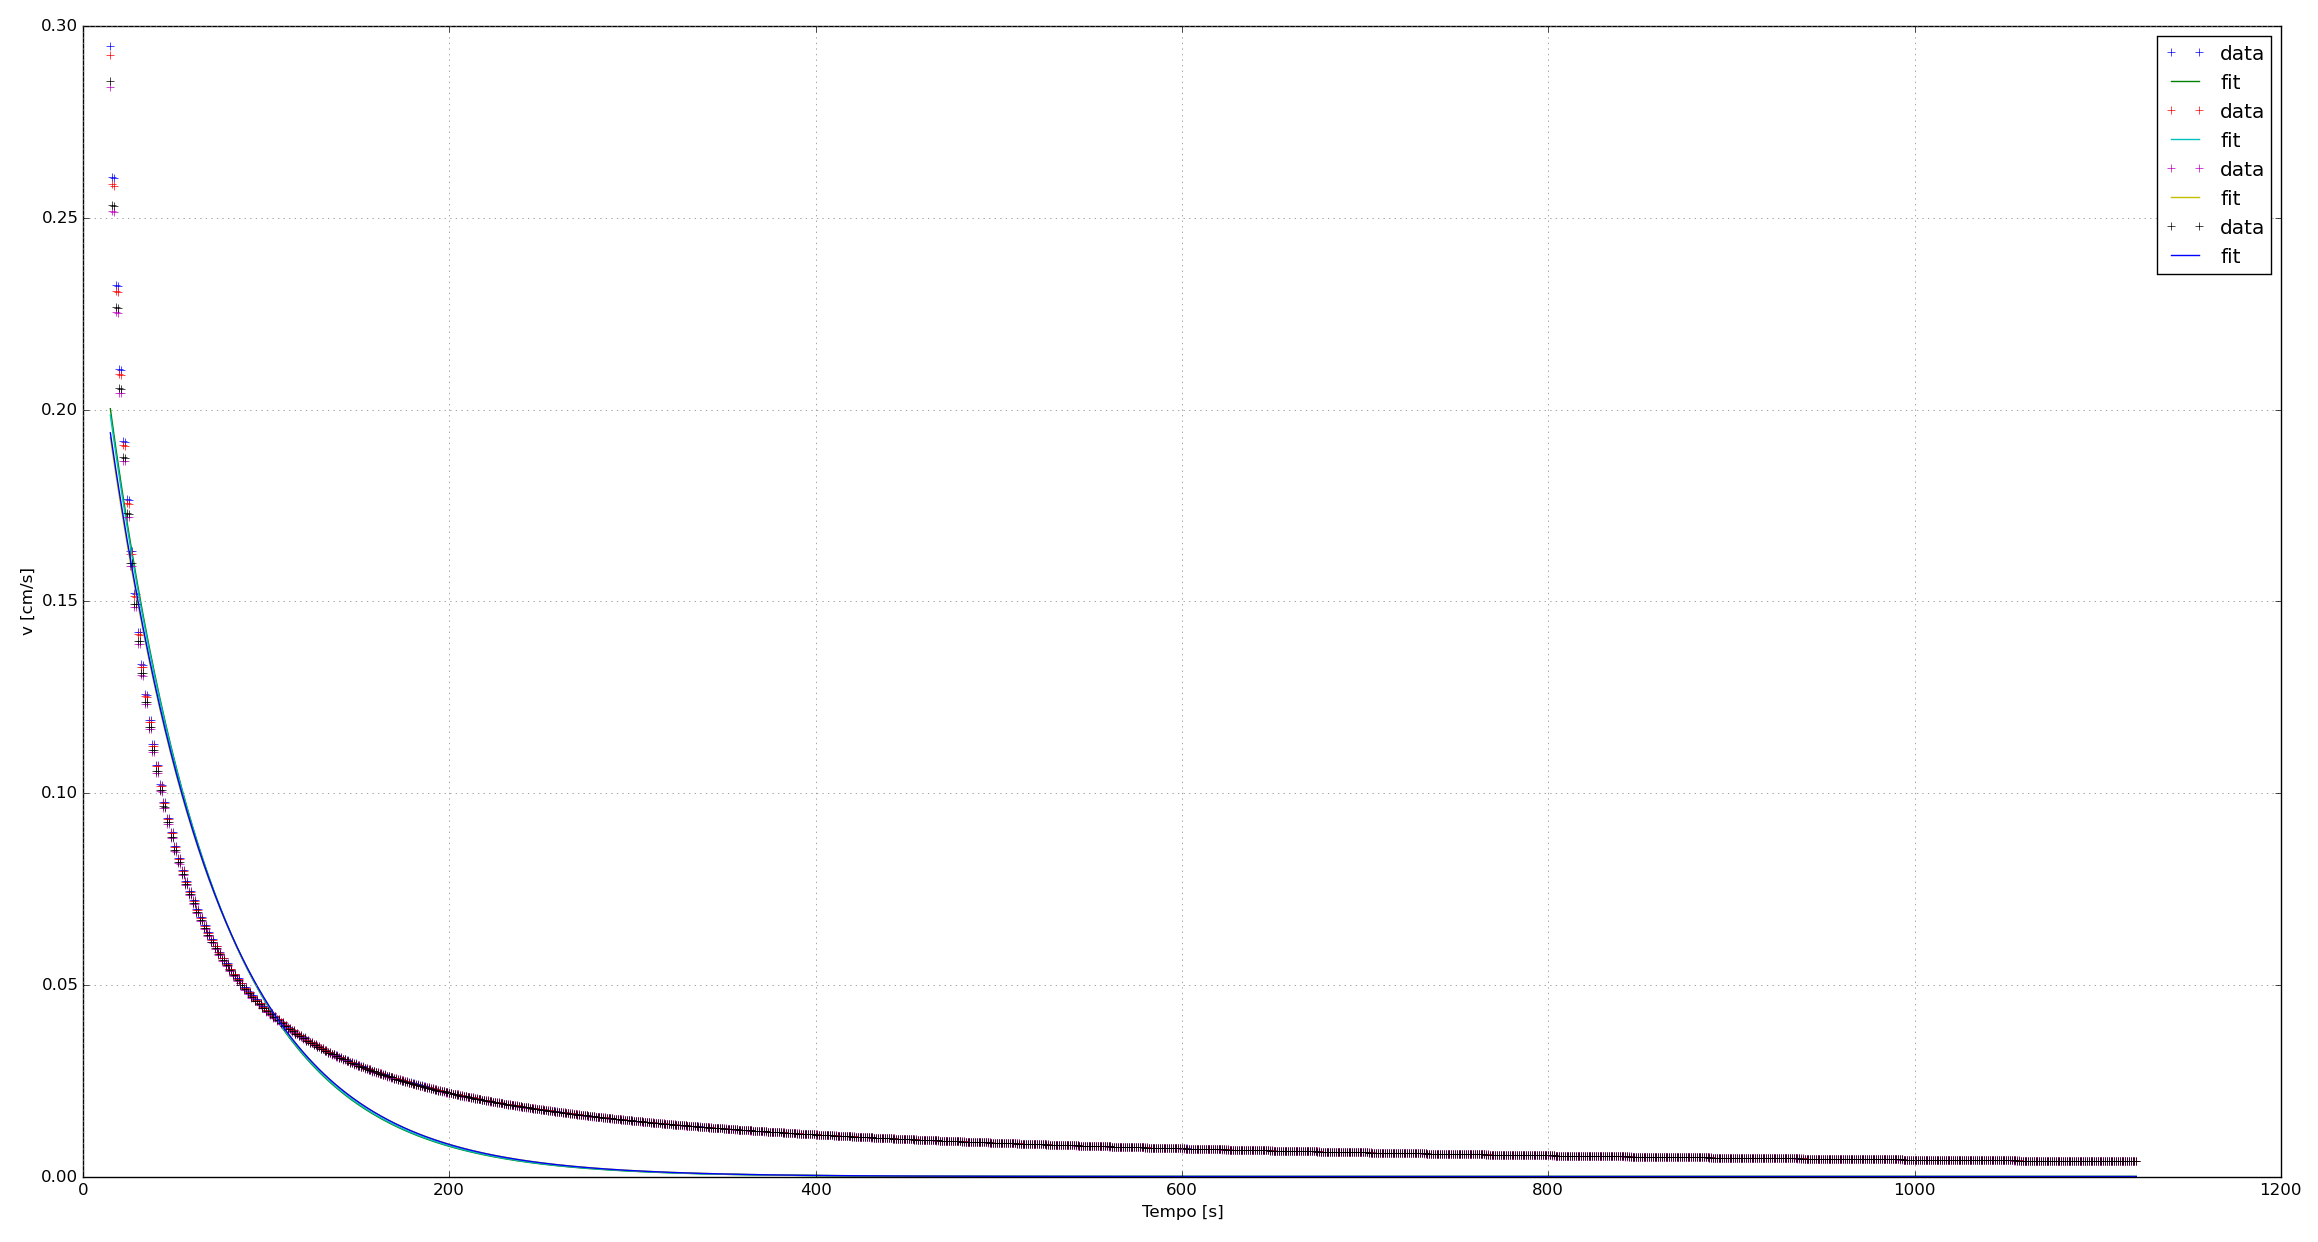
\includegraphics[width=10cm]{dati/pendolo4.png}
\end{center}
\end{figure}

Nel grafico possiamo osservare che il fit non approssima in maniera corretta i dati sperimentali.

\begin{figure}[!htb]
\begin{center}
\includegraphics[width=10cm]{dati/}
\end{center}
\end{figure}



\section{Conclusione}
Riguardo al grafico velocità-tempo siccome la presa dati è stata consistente possiamo concludere che il modello teorico non è del tutto corretto. Infatti il nostro modello considera
l'attrito come $k\dot{\theta}$ ma dai dati possiamo osservare che questo modello non è valido, tuttavia possiamo considerare attriti di diversa natura, bastando che compaiano in ordine dispari 
e superiore al primo nell'eqauzione differenziale del moto del pendolo. In questo modo dovremmo riuscire ad ottenere una migliore approssimazione.
\end{document}


